\documentclass[10pt,twocolumn]{article}

\usepackage[T1]{fontenc}
\usepackage[utf8]{inputenc}
\usepackage{lmodern}
\usepackage[a4paper,margin=0.85in]{geometry}
\setlength{\columnsep}{0.28in}
\usepackage{amsmath,amssymb}
\usepackage{booktabs}
\usepackage{array}
\usepackage{longtable}
\usepackage{graphicx}
\usepackage{tikz}
\usetikzlibrary{arrows.meta,positioning,fit,backgrounds}
\usepackage{hyperref}
\hypersetup{
  colorlinks=true,
  linkcolor=black,
  citecolor=black,
  urlcolor=blue,
  pdftitle={ReproBot -- First Progress Report},
  pdfauthor={Aleyna Kütük, Engincan Varan, Gül Korkut, Göktuğ Mert Özdoğan}
}
\usepackage{xcolor}
\usepackage{caption}
\usepackage{pifont}

\title{\textbf{ReproBot: A Multi-Agent System for Automated Scientific Paper Replication}\\[0.4em]
\large First Progress Report}
\author{
  Aleyna Kütük \\ \small\texttt{aleynakutuk10@gmail.com}
  \and
  Engincan Varan \\ \small\texttt{engincanvaran@gmail.com}
  \and
  Gül Korkut \\ \small\texttt{serifegulkorkut@gmail.com}
  \and
  Göktuğ Mert Özdoğan \\ \small\texttt{goekmeroz@gmail.com}
}
\date{inzva AI Projects \#10 \\ 17.07.2026}

\begin{document}

\maketitle

\begin{abstract}
Reproducing the empirical results of a machine learning paper remains a largely manual,
labor-intensive task, with the large majority of published work shipping no usable
implementation at all. \textbf{ReproBot} is a proposed multi-agent pipeline that reads
an ML paper in PDF form, extracts its method and claims, generates and executes a
training script, and produces a structured report comparing reproduced metrics against
the paper's stated numbers -- retrying the implementation when a Critic agent detects a
mismatch. This document reports on the project's first phase: a literature review of
nine closely related agentic-ML and paper-replication systems, a detailed
implementation-ready project plan (architecture, agent specifications, evaluation
rubric, timeline, risk register, and cost budget), and an early prototype of the Reader
agent that drafts method summaries, claims, and hyperparameters from paper PDFs using the
Anthropic API together with \texttt{pdfplumber}-based text extraction -- so far tried only
on a small sample of CIFAR-10 papers. We summarize what has been completed, what remains
open, and the concrete next steps for maturing the Reader and beginning the Coder and
Runner components.
\end{abstract}

\section{Introduction and Motivation}
\label{sec:intro}

Reproducing the empirical results of a machine learning paper is, in principle, a
mechanical exercise: read the method, implement it, run it, and compare the numbers.
In practice it is one of the most labor-intensive tasks in ML research. A reader must
reconstruct architectural details that authors often under-specify, infer
hyperparameters and data-processing conventions treated as ``common knowledge'' within a
subfield, and debug an implementation against a single, sparse signal -- whether the
final reported metric matches. The problem is compounded by how rarely authors release
usable code: across ICLR, ICML, and NeurIPS 2024, only 16.7--21.2\% of accepted papers
shipped a working implementation \cite{seo2025papercoder}, leaving the large majority of
the field's claims effectively unverifiable without a from-scratch reimplementation.

Large language model (LLM) agents have, over the last two years, been applied to nearly
every stage of this problem individually: benchmarked on general ML experimentation
\cite{huang2023mlagentbench}, tasked with generating entirely new research ideas and
writing them up as papers \cite{lu2024aiscientist,li2024mlrcopilot}, and used as coding
assistants that translate a paper's method section into a code repository
\cite{seo2025papercoder}. A rigorous benchmark now exists for measuring paper-replication
capability directly, complete with author-validated grading rubrics
\cite{starace2025paperbench}. Yet across this body of work, a specific combination of
capabilities -- parsing a paper's claims, executing a faithful implementation, and
explicitly verifying that the reproduced numbers match what was published, with an
iterative repair loop driven by that comparison -- has not been assembled into a single
system (Section~\ref{sec:related}).

\textbf{ReproBot} targets exactly this combination. It is structured as a four-agent
pipeline -- Reader, Coder, Runner, and Critic -- coordinated by a central Orchestrator
over a shared memory state (Section~\ref{sec:architecture}). The Reader ingests a paper
PDF and extracts a structured method summary, claims, datasets, and hyperparameters; the
Coder translates this into a self-contained HuggingFace \texttt{Trainer}-based training
script; the Runner executes the script in an isolated sandbox and captures metrics and
error traces; and the Critic compares the reproduced metrics against the paper's stated
numbers, producing a pass/retry/fail verdict and, on retry, targeted feedback for the
Coder. The pipeline is deliberately scoped at launch to a benchmark of 20
image-classification papers, trading the topic breadth of general-purpose benchmarks for
a tighter, more auditable definition of ``replication success'' within a single,
well-understood domain.

This report covers the project's first phase of work: literature review, detailed
planning, and an early Reader agent prototype. Section~\ref{sec:related} reviews the
related work that shaped ReproBot's design. Section~\ref{sec:architecture} describes the
proposed architecture. Section~\ref{sec:evaluation} describes the evaluation
methodology. Section~\ref{sec:timeline} lays out the project timeline.
Section~\ref{sec:progress} is the core contribution of this report: a concrete account
of what has been completed to date and what remains open. Section~\ref{sec:next}
describes next steps, and Section~\ref{sec:conclusion} concludes.

\section{Related Work}
\label{sec:related}

\subsection{Foundations: Benchmarking Agentic ML Experimentation}

The starting point for this line of work is \textbf{MLAgentBench}
\cite{huang2023mlagentbench}, the first benchmark to measure whether LLM agents can
conduct open-ended ML experimentation rather than merely propose hyperparameters. It
poses 13 executable tasks -- spanning canonical benchmarks (CIFAR-10, IMDB sentiment),
classic Kaggle competitions, and research-recency-controlled challenges -- and scores an
agent's final submission against a starter-code baseline. Its agent architecture, a
ReAct-style loop augmented with explicit Reflection, Research-Plan-and-Status, and
Fact-Check fields, targets two failure modes the authors identify as central to agentic
ML work: poor long-horizon planning and hallucinated progress claims. Even so, the
best-performing configuration (Claude 3 Opus) reaches only a 37.5\% average success rate
across the 13 tasks.

MLAgentBench does not ask an agent to read a paper at all, let alone reproduce one; its
contribution to ReproBot is architectural. The finding that unstructured agent loops
hallucinate and lose the plot over long horizons directly motivates separating concerns
across a Reader, Coder, Runner, and Critic under a single Orchestrator, rather than
asking one agent to do everything.

\subsection{The Detour Through Autonomous Research Generation}

Rather than pursuing replication, the field's next wave of systems pointed LLM agents at
generating \emph{new} research. \textbf{The AI Scientist} \cite{lu2024aiscientist} was
the first to close a full loop -- idea generation, iterative experimentation, manuscript
writing, and automated peer review -- end to end, at a reported cost of roughly \$10--15
per paper, but is candid about failure modes directly relevant to any autonomous
verification system: models fabricated ablation tables and mischaracterized a regressed
metric as an improvement. \textbf{The AI Scientist-v2} \cite{yamada2025aiscientistv2}
replaced linear iteration with a stage-gated tree search and added a vision-language
model (VLM) critic over generated figures; one of its fully autonomous submissions was
accepted to an ICLR 2025 workshop, though the authors note the other two were rejected.

\textbf{MLR-Copilot} \cite{li2024mlrcopilot} retrieves prototype code and candidate
models/datasets directly from HuggingFace rather than generating everything from a blank
context, and its cleanest empirical result is directly relevant to ReproBot: a
single-shot code-generation baseline succeeds on \textbf{0\% of trials} across all five
evaluated tasks, while its full iterative debugging loop reaches up to 50\% success with
the strongest backbone tested -- quantified evidence that iterative repair, not just code
generation, is what makes autonomous implementation viable at all.
\textbf{Agent Laboratory} \cite{schmidgall2025agentlab} rounds out this wave with a
three-phase pipeline and a configurable human-in-the-loop mode; its own automated
reviewer scores generated papers at 6.1/10 on average versus 3.8/10 from real human
reviewers -- a 2.3-point overestimation that argues against trusting any pipeline's
self-assessment of its own output without an independent, objective check.

This wave demonstrates that LLM agents can execute the entire research lifecycle end to
end, but leaves the replication problem untouched by construction -- these systems have
no ground-truth number to reproduce, since they invent the research question themselves.
They remain complementary to ReproBot, and several of their components -- Agent
Laboratory's code-mutation loop with pooled scoring, MLR-Copilot's
retrieve-then-integrate pattern, and The AI Scientist-v2's stage-gated tree search --
are directly transferable design patterns for ReproBot's own Coder and Critic loop.

\subsection{The Replication Wave: Benchmarks and Systems}
\label{sec:replication-wave}

A third, more recent wave of work returns to the narrower problem ReproBot targets
directly: given an existing paper, can an agent reproduce it. \textbf{PaperBench}
\cite{starace2025paperbench} is the field's gold-standard evaluation instrument. It
gives agents 20 ICML 2024 Spotlight/Oral papers and requires a from-scratch code
repository, graded against a hierarchical rubric of 8,316 individually gradable
leaf-node outcomes split into Code Development, Execution, and Result Match categories.
A human baseline shows PhD-level researchers start slower than the best agent
configuration but overtake it after roughly 24 hours of sustained work, suggesting
current agents plateau on long-horizon tasks rather than lacking raw capability.

\textbf{PaperCoder} \cite{seo2025papercoder} decomposes paper-to-code translation into
Planning, Analysis, and Coding stages, generating files sequentially in a
dependency-aware order. On PaperBench's lightweight Code-Dev variant it reaches a 45.1\%
replication score -- roughly double the best flat-ReAct baseline -- but it
\textbf{never executes} the code it produces; its own coverage analysis identifies data
processing as the weakest-implemented component (56\% coverage versus 79--92\%
elsewhere), precisely because papers are least explicit about data handling and no
execution step exists to surface the gap.

\textbf{AutoP2C} \cite{lin2025autop2c} closes the execution gap PaperCoder leaves open by
treating paper-to-code as an explicitly multimodal task -- parsing prose, equations,
tables, and, via a VLM, architecture diagrams -- and iteratively debugging the generated
code (execute $\to$ localize error $\to$ correct $\to$ repeat) until it runs. It reports
the strongest executability numbers surveyed (100\% of 8 benchmark papers produce
runnable code, versus 12.5\% for single-pass o1/DeepSeek-R1 baselines) and an ablation
showing that removing architecture-diagram parsing alone costs 21.9 points of absolute
reproduced performance. Its one quantitative ground-truth comparison -- average
``relative performance'' of 99.5\% -- is, however, an aggregate figure with
\textbf{no stated tolerance or pass/fail criterion}.

\textbf{AutoReproduce} \cite{zhao2025autoreproduce} introduces the \emph{paper lineage}
algorithm: mining a paper's citation graph for the papers it most heavily builds on and
using their text and linked code as grounding context during generation, paired with a
sampling-based unit-testing strategy that dry-runs a training script on a mini-batch
before committing to a full run. This dry-run technique alone was the single largest
driver of their execution-rate improvement (roughly 2--23\% for non-lineage baselines up
to 77--95\% with lineage). Yet AutoReproduce's headline metric is execution rate and
performance gap against a \emph{reference implementation}, not an explicit comparison
against the paper's own claimed numbers.

\subsection{The Gap ReproBot Fills}

Read together, the replication wave traces a clean division of labor with one piece
missing. PaperCoder proves a paper's method can become structurally coherent code, but
the code is never run. AutoP2C closes the execution gap and adds multimodal parsing,
coming closest to ReproBot's own pipeline shape -- but its debugging loop terminates on
``the code runs and looks architecturally aligned,'' with no stated tolerance on its one
ground-truth comparison.

AutoReproduce runs the code and improves on PaperCoder's benchmark scores via
citation-lineage mining, but its success criterion stops at executability and
reference-code similarity, not a direct comparison to the paper's stated claims.
\textbf{None of the three closes the loop from reproduced metric to an explicit pass/fail
verdict against the published number to a targeted retry.} Table~\ref{tab:gap} makes this
concrete across six capabilities: ReproBot is the only system that covers all six.

\begin{table*}[t]
\centering
\small
\setlength{\tabcolsep}{4pt}
\renewcommand{\arraystretch}{1.15}
\begin{tabular}{@{}l*{6}{c}@{}}
\toprule
\textbf{System} & \textbf{PDF+VLM} & \textbf{Code} & \textbf{Code} & \textbf{Metric} &
\textbf{Critic} & \textbf{Struct.} \\
& \textbf{parsing} & \textbf{gen.} & \textbf{exec.} & \textbf{vs.\ claim} &
\textbf{loop} & \textbf{report} \\
\midrule
MLAgentBench (2023)      & \ding{55} & $\sim$ & \ding{51} & \ding{55} & $\sim$ & \ding{55} \\
PaperBench (2025)        & \ding{51} & \ding{51} & \ding{51} & $\sim$ & $\sim$ & \ding{55} \\
PaperCoder (2025)        & \ding{51} & \ding{51} & \ding{55} & \ding{55} & \ding{55} & $\sim$ \\
AutoP2C (2025)           & \ding{51} & \ding{51} & \ding{51} & $\sim$ & $\sim$ & \ding{55} \\
AutoReproduce (2025)     & \ding{51} & \ding{51} & \ding{51} & \ding{55} & $\sim$ & \ding{55} \\
Agent Laboratory (2025)  & $\sim$ & \ding{51} & \ding{51} & \ding{55} & \ding{51} & \ding{51} \\
AI Scientist v1/v2 (2024)& \ding{55}/$\sim$ & \ding{51} & \ding{51} & \ding{55} & \ding{51} & \ding{51} \\
MLR-Copilot (2024)       & \ding{55} & \ding{51} & \ding{51} & \ding{55} & $\sim$ & \ding{55} \\
\midrule
\textbf{ReproBot (ours)} & \ding{51} & \ding{51} & \ding{51} & \ding{51} & \ding{51} & \ding{51} \\
\bottomrule
\end{tabular}
\caption{Capability gap matrix across replication and research-generation systems.
\ding{51} = full support, $\sim$ = partial, \ding{55} = not supported. The critical
missing column in every prior system is \emph{metric vs.\ claim} paired with a Critic
retry loop -- exactly what ReproBot adds. The specific design choices borrowed from each
system are detailed in Section~\ref{sec:architecture}.}
\label{tab:gap}
\end{table*}

\section{Proposed System Architecture}
\label{sec:architecture}

ReproBot is structured as a four-agent pipeline coordinated by a central
\textbf{Orchestrator} that owns a single, versioned shared-memory object per paper
(Figure~\ref{fig:pipeline}).

\begin{figure*}[t]
\centering
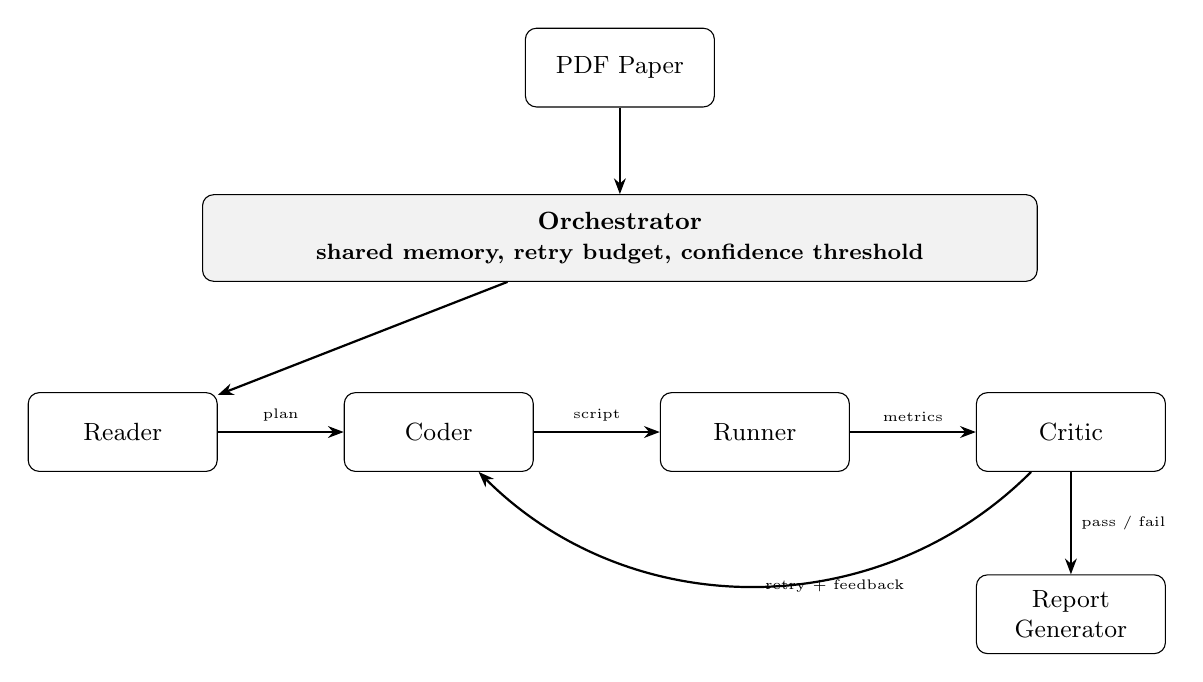
\begin{tikzpicture}[
  node distance=1.1cm and 1.6cm,
  box/.style={draw, rounded corners, minimum width=2.4cm, minimum height=1cm,
    align=center, font=\small},
  orch/.style={draw, rounded corners, minimum width=10.6cm, minimum height=1.1cm,
    align=center, font=\small\bfseries, fill=gray!10},
  arr/.style={-{Stealth[length=2mm]}, thick}
]
  \node[box] (pdf) {PDF Paper};
  \node[orch, below=of pdf] (orchestrator) {Orchestrator\\ \footnotesize shared memory, retry budget, confidence threshold};
  \node[box, below left=1.4cm and -0.2cm of orchestrator] (reader) {Reader};
  \node[box, right=of reader] (coder) {Coder};
  \node[box, right=of coder] (runner) {Runner};
  \node[box, right=of runner] (critic) {Critic};
  \node[box, below=1.3cm of critic] (report) {Report\\Generator};

  \draw[arr] (pdf) -- (orchestrator);
  \draw[arr] (orchestrator) -- (reader);
  \draw[arr] (reader) -- node[above,font=\tiny]{plan} (coder);
  \draw[arr] (coder) -- node[above,font=\tiny]{script} (runner);
  \draw[arr] (runner) -- node[above,font=\tiny]{metrics} (critic);
  \draw[arr] (critic) to[bend left=45] node[right,font=\tiny]{retry + feedback} (coder);
  \draw[arr] (critic) -- node[right,font=\tiny]{pass / fail} (report);
\end{tikzpicture}
\caption{ReproBot pipeline. The Orchestrator drives the Reader $\to$ Coder $\to$ Runner
$\to$ Critic loop until results clear a confidence threshold or the retry budget is
exhausted, then hands off to the Report Generator.}
\label{fig:pipeline}
\end{figure*}

\begin{itemize}
  \item \textbf{Reader.} Ingests a PDF using \texttt{pdfplumber} (text/tables) and a
  vision-language model (figure/diagram parsing) to extract a method summary, claims
  (metric, dataset, reported value, source location), hyperparameters, and a dedicated
  data-processing pass -- data-processing detail is the single weakest-covered aspect of
  paper-to-code extraction across every surveyed system (56\% coverage in PaperCoder vs.\
  79--92\% elsewhere \cite{seo2025papercoder}), so it is treated as a first-class output
  field rather than folded into the general method summary.
  \item \textbf{Coder.} Translates the Reader's output into a self-contained HuggingFace
  \texttt{Trainer}-based training script; on retry, applies the Critic's targeted
  feedback rather than regenerating from scratch, following MLR-Copilot's
  retrieve-before-generate pattern for models and datasets \cite{li2024mlrcopilot}.
  \item \textbf{Runner.} Executes the script inside a Docker sandbox with no host
  access, cheaply validating it first with AutoReproduce's sampling-based dry run
  (mini-batch shape check + early-exit full-pipeline pass) before committing to a full
  training run \cite{zhao2025autoreproduce} -- this technique alone drove that system's
  largest execution-rate gains.
  \item \textbf{Critic.} Compares the Runner's reproduced metrics against the Reader's
  extracted claims and produces a structured \texttt{pass}/\texttt{retry}/\texttt{fail}
  verdict with an explicit numeric tolerance, plus targeted natural-language feedback on
  retry -- the tolerance gate that Section~\ref{sec:replication-wave} identifies as
  missing from every surveyed replication system.
  \item \textbf{Orchestrator.} Owns the shared-memory object, enforces the retry budget
  and confidence threshold, and checks the append-only history log before each retry to
  avoid burning the budget on a plateaued fix.
\end{itemize}

Model selection standardizes on the Claude family: Claude Sonnet~5 as the default
backbone for the Reader, Coder, Critic, and Report Generator, with Claude Opus~4.8
reserved for low-confidence extractions, stuck retries (2+ failed attempts), and
borderline numeric judgment calls, and Claude Haiku~4.5 for cheap, high-volume
classification (Runner outcome triage, Orchestrator edge-case routing). This choice is
grounded directly in PaperBench's own backbone comparison, where Claude 3.5 Sonnet was
the clear leader among tested models (21.0\% average replication score vs.\ GPT-4o's
4.1\% and o1's 13.2\%) on exactly this kind of paper-comprehension-and-agentic-coding
task \cite{starace2025paperbench}.

\section{Evaluation Methodology}
\label{sec:evaluation}

The four replication-focused systems reviewed in Section~\ref{sec:replication-wave}
each invented their own evaluation vocabulary. Table~\ref{tab:rubric} maps these onto a
shared taxonomy and proposes a combined rubric for ReproBot's Critic: PaperBench's
three-tier taxonomy is adopted as the skeleton (it is the most validated, with an
author-co-developed rubric and a judge-reliability meta-check reaching F1~=~0.83
\cite{starace2025paperbench}), filled with the cheaper, more mechanistic techniques the
other systems proved effective, plus the one thing none of them define: an explicit
numeric tolerance gate.

\begin{table*}[t]
\centering
\small
\begin{tabular}{@{}p{2.4cm}p{3.6cm}p{5.6cm}p{2.2cm}@{}}
\toprule
\textbf{Tier} & \textbf{What it checks} & \textbf{Borrowed technique} & \textbf{Output} \\
\midrule
Code Development & Does the script structurally implement the method? & Component-coverage check by section (method / data-processing / eval) &
partial-credit \% \\
Execution & Does it run, cheaply verified before a full run? & Sampling-based dry-run (mini-batch check + early-exit pipeline pass) &
binary + triage class \\
Result Match & Does the reproduced metric match the paper's claim? & Continuous gap signal feeding an explicit numeric tolerance threshold &
pass / retry / fail \\
Meta-layer & Is the Critic's own judgment trustworthy? & Validate Critic feedback against a small hand-graded gold set &
judge F1 / correlation \\
\bottomrule
\end{tabular}
\caption{Proposed combined evaluation rubric for ReproBot's Critic agent.}
\label{tab:rubric}
\end{table*}

Success will be reported along three axes rather than a single aggregate replication
rate: \textbf{coverage} (how many target papers produced any executing script),
\textbf{fidelity} (of those, how many reproduced the claimed metric within the stated
tolerance, with the actual gap percentage reported per paper), and, as the headline
result, an \textbf{ablation} of replication rate with the Critic-driven retry loop
enabled versus disabled (single-shot Coder only) -- isolating the specific contribution
the literature review identifies as ReproBot's gap-filling feature.

\section{Project Timeline}
\label{sec:timeline}

The original proposal laid out four monthly milestones: Reader (Month~1), Coder~+~Runner~+
Orchestrator skeleton (Month~2), Critic~+~refinement loop~+~report generation (Month~3),
and evaluation~+~ablation~+~demo (Month~4). Detailed planning (Section~\ref{sec:progress})
refined this into the staged breakdown in Table~\ref{tab:timeline}, with an explicit pilot
checkpoint -- validating the pipeline end to end on 3--5 papers -- before committing to
the full 20-paper benchmark.

\begin{table*}[t]
\centering
\small
\begin{tabular}{@{}p{2.6cm}p{12.4cm}@{}}
\toprule
\textbf{Phase} & \textbf{Focus} \\
\midrule
Month 1 & PDF ingestion, Reader prompt/schema design, shared-memory object definition;
Reader validated on 3--5 pilot papers. \\
Month 2 & Coder generating scripts for the pilot set; Docker sandbox with sampling-based
dry-run validation; Orchestrator skeleton (Reader $\to$ Coder $\to$ Runner) with a
hard-coded single retry. \\
Month 3 & Critic verdict logic (pass/retry/fail + three-way Execution/Code-Dev/Result-Match
split); real retry loop with targeted feedback; Report Generator; single-shot vs.\
iterative-loop ablation on the pilot set. \\
Month 4 & Expand from the pilot set toward the full 20-paper target as compute/time
allows; Gradio demo; ablation write-up; final project report. \\
\bottomrule
\end{tabular}
\caption{Revised, staged project timeline.}
\label{tab:timeline}
\end{table*}

\section{Progress to Date}
\label{sec:progress}

This section is the core contribution of the present report: a concrete account of what
has been completed since the project proposal, and what remains open.

\subsection{Completed: Literature Review}

Nine closely related systems were surveyed in depth and organized into three internal
documents that serve different purposes: a cross-paper comparison document with a
landscape diagram, a chronological wave structure, per-paper architecture deep dives,
and a capability gap matrix; a template-consistent per-paper summary document preserving
exact reported numbers (success rates, replication scores, costs) for later citation;
and a polished prose draft of the Introduction and Literature Review sections, ready to
be copy-edited into the final project report (Section~\ref{sec:related} of this document
is drawn directly from it). A companion evaluation-metrics comparison document
(Section~\ref{sec:evaluation}) inventories every metric these four replication-focused
papers report, checks judge/grader trustworthiness, and proposes the combined rubric
ReproBot's Critic will use.

\subsection{Completed: Detailed Project Plan}

Beyond the original proposal, a detailed, implementation-ready project plan was
produced, covering: a feasibility assessment grounded in comparable systems' actual
reported numbers (Table~\ref{tab:reality-check} reproduces the key comparison); an
architecture deep dive with the concrete shared-memory JSON schema threaded through every
agent call; per-agent specifications (responsibilities, tools, recommended model,
literature-grounded risks and mitigations); the revised staged timeline in
Section~\ref{sec:timeline}; a risk register; and a rough compute/cost budget.

\begin{table*}[t]
\centering
\small
\begin{tabular}{@{}p{3.2cm}p{4cm}p{4.8cm}p{2.8cm}@{}}
\toprule
\textbf{System} & \textbf{Team / effort} & \textbf{What they achieved} & \textbf{Cost} \\
\midrule
PaperBench BasicAgent & Dedicated OpenAI team & 21.0\% avg.\ replication score
(Claude 3.5 Sonnet), 20 ICML papers & $\sim$\$400/paper + \$66/paper grading \\
PaperCoder & Research team, months & 45.1\% on Code-Dev (no execution); 28.5\% on
execution+result-match subset & Not reported \\
AutoReproduce & Research team & 48.5\% on Code-Dev with lineage; 77--95\% execution rate
on own benchmark & Not reported \\
Human ML PhDs & 8 PhDs, 48h each & $\sim$41.4\% best-of-3 & N/A \\
\bottomrule
\end{tabular}
\caption{Reality check against comparable systems -- no reviewed system reaches close to
faithful replication, which frames the 20-paper benchmark as a demonstration of the
retry-loop contribution rather than a claim to beat these numbers.}
\label{tab:reality-check}
\end{table*}

\subsection{Early Prototyping: Reader Agent}

An early prototype of the \textbf{Reader} agent has been sketched out, but it is at a
very preliminary stage. It uses \texttt{pdfplumber} to extract text from a paper PDF and
the Anthropic API (Claude) to draft a mostly-structured method summary, claims, and
hyperparameters from that text.

So far it has only been tried on a small handful of CIFAR-10 image-classification papers
(ResNet, DenseNet, and similar canonical architectures) -- deliberately chosen to match
the project's launch domain. This is a first sanity check of the extraction idea, not a
validated component: no systematic accuracy evaluation has been run, the output schema is
not yet reliably machine-parseable, and the vision-language component for figures,
diagrams, and tables is not yet integrated (the prototype relies on \texttt{pdfplumber}
text alone).

AutoP2C's ablation is a direct reminder that the VLM piece matters: removing
architecture-diagram parsing alone cost 21.9 points of absolute reproduced performance in
their evaluation \cite{lin2025autop2c}. Hardening the schema and adding VLM-based figure
parsing are therefore near-term priorities, not optional enhancements.

\subsection{Not Yet Started}

The Coder, Runner, and Critic agents, the Orchestrator's shared-memory state machine, the
Docker sandbox, and the report generator have not yet been implemented. No pilot-paper
validation (the 3--5 paper checkpoint in Table~\ref{tab:timeline}) has been run yet, and
consequently no reproduced metrics, executability rates, or ablation results exist at
this stage. The project team has also grown from the two authors on the original
proposal to four members (Aleyna Kütük, Engincan Varan, Gül Korkut, Göktuğ Mert
Özdoğan), which has not yet been reflected in a revised division of labor beyond the
initial kickoff presentation.

\section{Next Steps}
\label{sec:next}

The immediate priorities, in order, are:
\begin{enumerate}
  \item \textbf{Harden the Reader's extraction schema} so that method summary, claims
  (with explicit source location), hyperparameters, and a dedicated data-processing
  field are all reliably machine-parseable, and validate it by hand against 3--5 pilot
  papers as specified in the project plan.
  \item \textbf{Add VLM-based figure and table parsing} to the Reader, given the
  concrete evidence in Section~\ref{sec:replication-wave} that this materially affects
  reproduced performance.
  \item \textbf{Define the shared-memory schema in code} and stand up a minimal
  Orchestrator skeleton that can pass the Reader's output to a (initially stubbed)
  Coder.
  \item \textbf{Begin the Coder agent}, targeting a single self-contained HuggingFace
  \texttt{Trainer} script per paper, and the Docker sandbox with the sampling-based
  dry-run check built first.
  \item Finalize the division of labor across the now four-person team against the
  agent specifications in Section~\ref{sec:architecture}.
\end{enumerate}

\section{Conclusion}
\label{sec:conclusion}

This report covers ReproBot's first phase of work: a literature review of nine closely
related agentic-ML and paper-replication systems, a detailed implementation-ready
project plan, and an early prototype of the Reader agent. The literature review confirms
a specific, well-evidenced gap -- no surveyed system closes the loop from a reproduced
metric to an explicit pass/fail verdict against the paper's own claim to a targeted
retry -- that ReproBot's Critic-driven design is intended to fill.

Implementation is still at an early stage. The Reader prototype has only been tried on a
small sample of CIFAR-10 papers and is not yet schema-complete or multimodal, and the
Coder, Runner, Critic, and Orchestrator remain to be built. The next phase focuses on
maturing and validating the Reader against the pilot paper set before extending the
pipeline to code generation and execution.

\bibliographystyle{plain}
\begin{thebibliography}{9}

\bibitem{huang2023mlagentbench}
Huang, Q., Vora, J., Liang, P., \& Leskovec, J. (2023).
MLAgentBench: Evaluating Language Agents on Machine Learning Experimentation.
\textit{arXiv:2310.03302}.

\bibitem{starace2025paperbench}
Starace, G., Jaffe, O., Sherburn, D., Aung, J., et al. (2025).
PaperBench: Evaluating AI's Ability to Replicate AI Research.
\textit{arXiv:2504.01848}.

\bibitem{seo2025papercoder}
Seo, M., Baek, J., Lee, S., \& Hwang, S.~J. (2025).
Paper2Code: Automating Code Generation from Scientific Papers in Machine Learning.
\textit{arXiv:2504.17192} (ICLR 2026).

\bibitem{lin2025autop2c}
Lin, Z., Shen, Y., Cai, Q., Sun, H., Zhou, J., \& Xiao, M. (2025).
AutoP2C: An LLM-Based Agent Framework for Code Repository Generation from Multimodal
Content in Academic Papers.
\textit{arXiv:2504.20115}.

\bibitem{zhao2025autoreproduce}
Zhao, X., Sang, Z., Li, Y., Shi, Q., et al. (2025).
AutoReproduce: Automatic AI Experiment Reproduction with Paper Lineage.
\textit{arXiv:2505.20662}.

\bibitem{schmidgall2025agentlab}
Schmidgall, S., Su, Y., et al. (2025).
Agent Laboratory: Using LLM Agents as Research Assistants.
\textit{arXiv:2501.04227}.

\bibitem{lu2024aiscientist}
Lu, C., Lu, C., Lange, R.~T., Foerster, J., Clune, J., \& Ha, D. (2024).
The AI Scientist: Towards Fully Automated Open-Ended Scientific Discovery.
\textit{arXiv:2408.06292}.

\bibitem{yamada2025aiscientistv2}
Yamada, Y., Lange, R.~T., Lu, C., et al. (2025).
The AI Scientist-v2: Workshop-Level Automated Scientific Discovery via Agentic Tree
Search.
\textit{arXiv:2504.08066}.

\bibitem{li2024mlrcopilot}
Li, R., Patel, T., Wang, Q., \& Du, X. (2024).
MLR-Copilot: Autonomous Machine Learning Research based on Large Language Models Agents.
\textit{arXiv:2408.14033}.

\end{thebibliography}

\end{document}
